\documentclass[12pt]{article}
\documentclass[12pt]{article}
\usepackage[utf8]{inputenc}
\usepackage[spanish]{babel}
\decimalpoint
\usepackage{amsmath}
\usepackage{amsthm}
\usepackage{amssymb}
\usepackage{graphicx}
\usepackage[margin=0.9in]{geometry}
\usepackage{fancyhdr}
\usepackage[inline]{enumitem}
\usepackage{float}
\usepackage{cancel}
\usepackage{bigints}
\usepackage{color}
\usepackage{xcolor}
\usepackage{listingsutf8}
\usepackage{algorithm}
\usepackage{tocloft}
\usepackage[none]{hyphenat}
\usepackage{graphicx}
\usepackage{grffile}
\usepackage{tabularx}
\usepackage[nottoc,notlot,notlof]{tocbibind}
\usepackage{times}
\usepackage{color}
\definecolor{gray97}{gray}{.97}
\definecolor{gray75}{gray}{.75}
\definecolor{gray45}{gray}{.45}
\renewcommand{\cftsecleader}{\cftdotfill{\cftdotsep}}
\pagestyle{fancy}
\setlength{\headheight}{15pt} 
\lhead{Complejidad y análisis}
\rhead{\thepage}
\lfoot{ESCOM-IPN}
\renewcommand{\footrulewidth}{0.5pt}
\setlength{\parskip}{0.5em}
\newcommand{\ve}[1]{\overrightarrow{#1}}
\newcommand{\abs}[1]{\left\lvert #1 \right\lvert}
\date{06 de Septiembre 2018}
\title{Complejidad temporal y análisis de casos}
\author{Abigail Nicolás Sayago}

\definecolor{pblue}{rgb}{0.13,0.13,1}
\definecolor{pgreen}{rgb}{0,0.5,0}
\definecolor{pred}{rgb}{0.9,0,0}
\definecolor{pgrey}{rgb}{0.46,0.45,0.48}
\lstset{tabsize=1}

\usepackage{listings}
\lstset{ frame=Ltb,
framerule=0pt,
aboveskip=0.5cm,
framextopmargin=3pt,
framexbottommargin=3pt,
framexleftmargin=0.4cm,
framesep=0pt,
rulesep=.4pt,
backgroundcolor=\color{gray97},
rulesepcolor=\color{black},
%
stringstyle=\ttfamily,
showstringspaces = false,
basicstyle=\small\ttfamily,
commentstyle=\color{gray45},
keywordstyle=\bfseries,
%
numbers=left,
numbersep=15pt,
numberstyle=\tiny,
numberfirstline = false,
breaklines=true,
}

% minimizar fragmentado de listados
\lstnewenvironment{listing}[1][]
{\lstset{#1}\pagebreak[0]}{\pagebreak[0]}

\lstdefinestyle{consola}
{basicstyle=\scriptsize\bf\ttfamily,
backgroundcolor=\color{gray75},
}

\lstdefinestyle{Java}
{language=Java,
}

%%%%%%%%%%%%%%%%%%%%%

\lstdefinestyle{customc}{
  belowcaptionskip=1\baselineskip,
  breaklines=true,
  frame=L,
  xleftmargin=\parindent,
  language=C,
  showstringspaces=false,
  basicstyle=\footnotesize\ttfamily,
  keywordstyle=\bfseries\color{green!40!black},
  commentstyle=\itshape\color{purple!40!black},
  identifierstyle=\color{blue},
  stringstyle=\color{orange},
}

\lstdefinestyle{customasm}{
  belowcaptionskip=1\baselineskip,
  frame=L,
  xleftmargin=\parindent,
  language=[x86masm]Assembler,
  basicstyle=\footnotesize\ttfamily,
  commentstyle=\itshape\color{purple!40!black},
}

\lstset{escapechar=@,style=customc}

%Permite crear columnas en el documento
\usepackage{multicol} 
\usepackage{color}
\usepackage{comment}
\newcommand{\tabitem}{~~\llap{\textbullet}~~}
\newcommand{\subtabitem}{~~~~\llap{\textbullet}~~}

% ---------------------------------------------------
% 						FONT 
% ---------------------------------------------------

\usepackage{cmbright}								% Font


\begin{document}

% ###########################################################################################
% ----------------------------------- FANCY TITLE PAGE --------------------------------------
% ###########################################################################################
\begin{titlepage}
			\begin{center}
				\noindent
				\begin{minipage}{0.5\textwidth}
					\begin{flushleft} \large
						\includegraphics[width=0.7\textwidth]{../ipn.png}
					\end{flushleft}
				\end{minipage}%
				\begin{minipage}{0.55\textwidth}
					\begin{flushright} \large
						\includegraphics[width=0.5\textwidth]{../escom.png}
					\end{flushright}
				\end{minipage}
				
				\textsc{\LARGE Instituto Politécnico Nacional}\\[0.5cm]
				
				\textsc{\Large Escuela Superior de Cómputo}\\[1cm]
				
				% Title
				
				{ \huge Ejercicio 02 - Complejidad temporal y análisis de casos  \\[1cm] }
				
				{ \Large Unidad de aprendizaje: Teoría computacional} \\[1cm]
				
				{ \Large Grupo: 3CM3 } \\[1cm]
				
				\noindent
				\begin{minipage}{0.5\textwidth}
					\begin{flushleft} \large
						\emph{Alumno(a):}\\
						
						\begin{tabular}{ll}
					     Nicolás Sayago Abigail\\
					\end{tabular}
					\end{flushleft}
				\end{minipage}%
				\begin{minipage}{0.5\textwidth}
					\begin{flushright} \large
						\emph{Profesor(a):} \\
					    Edgardo Adrian Franco  \\
					\end{flushright}
				\end{minipage}
				
				\vfill
				
				% Bottom of the page
				{\large 06 Septiembre de 2018}
			\end{center}
		\end{titlepage}
	\tableofcontents
  \newpage
% ///////////////////////////////////////////////////////////////////////////
%									SECCIÓN A
% ///////////////////////////////////////////////////////////////////////////
	\section{Sección A}
	En esta sección se determinara la función de complejidad temporal y espacial en términos de n. Se consideran las operaciones de asignación, aritméticas, condicionales y saltos implícitos.

	% ----------------------------------------------------------------------
	% 															EJERCICIO 1
	% ----------------------------------------------------------------------
	    \subsection{Ejercicio 1}
	        \subsubsection{Algoritmo}
	        \begin{lstlisting}[style=Java]
for(i = 1; i < n; i++)
	for(j = 0; j <n-1; j++)
	{
		temp = A[j];
		A[j] = A[j+1];
		A[j+1] = temp;
	}

    		\end{lstlisting}

    		\subsubsection{Análisis}
    			\begin{itemize}
    				\item[\Checkmark] \textbf{Función temporal:} $f_{t}(n) = 8n^{2} - 10n +5$
    				\item[\Checkmark] \textbf{Función espacial:} $f_{e}(n) = n + 3$
    			\end{itemize}
    		\subsubsection{Código}
    		\begin{lstlisting}[style=Java]
#include <stdio.h>
#include <stdlib.h>

int main() {
  int i, j, n = 10, temp, A[n];
  int Funcion = 0, Contador = 0;
  Contador++; // Asignación
  for (i = 1; i < n; i++, Contador++) 
  {
    Contador++; // SALTO IMPLICITO - Cuando te dice que te vayas a dentro del FOR
    Contador++; // Comparacion que si se cumple
    Contador++; // Asignación de j = 0
    for (j = 0; j < n - 1; j++, Contador++) {
      Contador++; // SALTO IMPLICITO
      Contador++; // Comparacion
      Contador += 5; // operaciones
      temp = A[j];
      A[j] = A[j + 1];
      A[j + 1] = temp;
    }
    Contador++; // comparacion
    Contador++; // SALTO EN FALSO
  }
  Contador++; // Cuando comparas y no se cumple
  Contador++; // SALTO EN FALSO - Cuando no se cumple
  Funcion = 8*n*n-10*n+5;
  printf("# Funcion : %d \n", Funcion);
  printf("# Reales : %d", Contador);
  return 0;
}
    		\end{lstlisting}

    		\subsubsection{Capturas de prueba}
    			\begin{figure}[h!]
	                \centering
	                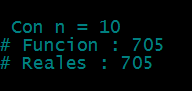
\includegraphics[width=\textwidth]{Abigail/Images/E1_1.PNG}
	 		    \end{figure} 

	% ----------------------------------------------------------------------
	% 															EJERCICIO 2
	% ----------------------------------------------------------------------
	    \subsection{Ejercicio 2}
		    \subsubsection{Algoritmo}
	        \begin{lstlisting}[style=Java]
polinomio = 0;
for(i = 0; i <= n; i++)
{
	polinomio = polinomio*z + A[n-i];
}
    		\end{lstlisting}

    		\subsubsection{Análisis}
    			\begin{itemize}
    				\item[\Checkmark] \textbf{Función temporal:} $f_{t}(n) = 7n + 11$
    				\item[\Checkmark] \textbf{Función espacial:} $f_{e}(n) = n + 3$
    			\end{itemize}
    		\subsubsection{Código}
    		\begin{lstlisting}[style=Java]
#include <stdio.h>
#include <stdlib.h>

int main() 
{
  int polinomio = 0, Funcion, i, n = 5000, z = 1, A[n];
  int Contador = 1;
  for (i = 0, Contador++; i <= n; i++, Contador++) 
  {
    Contador++; // SALTO IMPLICITO
    Contador += 4; // Numero de operaciones
    polinomio = polinomio * z + A[n - i];
    Contador++; // Numero de saltos
  }
  Contador++; // SALTO FALSO
  Contador++; // Compara y no es correcto
  Funcion = 7*n + 11;
  printf("\nCon n = %d \n", n); 
  printf("# por Funcion: %d \n", Funcion);
  printf("# de reales: %d \n", Contador);
}
	   		\end{lstlisting}

    		\subsubsection{Capturas de prueba}
				\begin{figure}[h!]
	                \centering
	                \includegraphics[width=\textwidth]{Abigail/Images/E2.PNG}
	 		    \end{figure} 
    		

   	% ----------------------------------------------------------------------
	% 															EJERCICIO 3
	% ----------------------------------------------------------------------
	    \subsection{Ejercicio 3}
	    	\subsubsection{Algoritmo}
	        \begin{lstlisting}[style=Java]
for(i = 1; i <= n; i++)
	for(j = 1; j <= n; j++)
		C[i,j] = 0;
		for(k = 1; k <= n; k++)
			C[i,j] = C[i,j] + A[i,k]*B[k,j]; 
    		\end{lstlisting}
    		\subsubsection{Análisis}
    			\begin{itemize}
    				\item[\Checkmark] \textbf{Función temporal:} $f_{t}(n) = 6n^{3} + 5n^{2} + 7n + 3 $
    				\item[\Checkmark] \textbf{Función espacial:} $f_{e}(n) = 3n^{2} + 3$
    			\end{itemize}
    		\subsubsection{Código}
    		\begin{lstlisting}[style=Java]
#include <stdio.h>
#include <stdlib.h>

int main() 
{
  int n = 4, Funcion = 0, Contador = 0;
  int i, j, k;
  for (i = 1, Contador++; i <= n; i++, Contador++) 
  {
    Contador++; // SALTO IMPLICITO
    for (j = 1, Contador++; j <= n; j++, Contador++) 
    {
      Contador++; // Comparacion
      Contador++; // Asignacion
      for (k = 1, Contador++; k <= n; k++, Contador++) 
      {
        Contador += 3; // Operaciones dentro del for
        Contador++; // Comparacion
      }
      Contador++;  // Comparacion
      Contador++;  // SALTO IMPLICITO
    }
    Contador++;  // Comparacion
    Contador++;  // SALTO IMPLICITO
  }
  Contador++; // Comparacion
  Contador++; // SALTO EXPLICITO
  Funcion = 6*n*n*n + 5*n*n + 7*n + 3;
  printf("\nCon n = %d \n", n); 
  printf("# por Funcion: %d \n", Funcion);
  printf("# de reales: %d \n", Contador);
  return 0;
}
	   		\end{lstlisting}

    		\subsubsection{Capturas de prueba}
				\begin{figure}[h!]
	                \centering
	                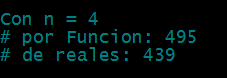
\includegraphics[width=\textwidth]{Abigail/Images/E3.PNG}
	 		    \end{figure} 

   	% ----------------------------------------------------------------------
	% 															EJERCICIO 4
	% ----------------------------------------------------------------------    
	    \subsection{Ejercicio 4}
	    	\subsubsection{Algoritmo}
	        \begin{lstlisting}[style=Java]
anterior = 1;
actual = 1;
while(n > 2)
{
	aux = anterior + actual;
	anterior = actual;
	actual = aux;
	n = n-1;
}
    		\end{lstlisting}
    		\subsubsection{Análisis}
    			\begin{itemize}
    				\item[\Checkmark] \textbf{Función temporal:} $f_{t}(n) =  $
    				\item[\Checkmark] \textbf{Función espacial:} $f_{e}(n) = 3$
    			\end{itemize}
    		\subsubsection{Código}
    		\begin{lstlisting}[style=Java]
#include <stdio.h>
#include <stdlib.h>

int main() 
{
  int anterior = 1;
  int actual = 1;
  int Funcion; 
  int n = 20, aux = 0;
  int Contador = 3;
  while (n > 2) 
  {
    Contador++;
    Contador++;
    aux = anterior + actual;
    anterior = actual;
    actual = aux;
    n = n - 1;
    Contador += 6;
  }
  Contador++;

  if(n <= 2)
    Funcion = 4;
  else
    Funcion = 8*n - 12;

  printf("\nCon n = %d \n", n); 
  printf("# por Funcion: %d \n", Funcion);
  printf("# de reales: %d \n", Contador);
  return 0;
}
	   		\end{lstlisting}

    		\subsubsection{Capturas de prueba}
				\begin{figure}[h!]
	                \centering
	                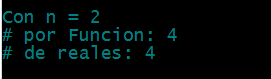
\includegraphics[width=\textwidth]{Abigail/Images/E4_1.PNG}
	 		    \end{figure} 

    % ----------------------------------------------------------------------
	% 															EJERCICIO 5
	% ----------------------------------------------------------------------
	    \subsection{Ejercicio 5}
	    	\subsubsection{Algoritmo}
	        \begin{lstlisting}[style=Java]
for(i = n -1; j = 0; i >= 0; i--, j++)
	s2[j] = s[i];

for(i = 0; i < n; i++)
	s[i] = s2[i];
    		\end{lstlisting}
    		\subsubsection{Análisis}
    			\begin{itemize}
    				\item[\Checkmark] \textbf{Función temporal:} $f_{t}(n) = 9n + 8 $
    				\item[\Checkmark] \textbf{Función espacial:} $f_{e}(n) = 2n + 2 $
    			\end{itemize}
    		\subsubsection{Código}
    		\begin{lstlisting}[style=Java]
#include <stdio.h>
#include <stdlib.h>

int main() 
{
  int n = 5, i = 0, j = 0, s[n], s2[n];
  int Contador = 0, Funcion;
  Contador += 4;
  for (i = n - 1, j = 0; i >= 0; i--, j++, Contador+=2)
  {
  	  s2[j] = s[i]; Contador++;
  	  Contador++;
  	  Contador++;
  }
  Contador++;

  Contador+=2; // Asignacion y caso no entra
  for (i = 0; i < n; i++,  Contador++)
  {
  	s[i] = s2[i];
  	Contador+=3;
  } 
  Contador++;
  	
  Funcion = 9*n +8;
  printf("\nCon n = %d \n", n); 
  printf("# por Funcion: %d \n", Funcion);
  printf("# de reales: %d \n", Contador);
  return 0;
}
	   		\end{lstlisting}

    		\subsubsection{Capturas de prueba}
				\begin{figure}[h!]
	                \centering
	                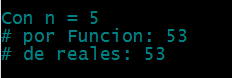
\includegraphics[width=\textwidth]{Abigail/Images/E5.PNG}
	 		    \end{figure} 

\newpage
% ///////////////////////////////////////////////////////////////////////////
%									SECCIÓN B
% ///////////////////////////////////////////////////////////////////////////	
	\section{Sección B}
	Para los siguiente 3 algoritmos se determinara el número de veces que imprime la palabra "Algoritmos". 

    % ----------------------------------------------------------------------
	% 															EJERCICIO 6
	% ----------------------------------------------------------------------
	    \subsection{Ejercicio 6}
			\subsubsection{Algoritmo}	    
    			\begin{lstlisting}[style=Java]
for(i = 10; i < n*5; i *= 2)
	printf("\"Algoritmos\n\"");    		    
    			\end{lstlisting}
    		
    		\subsection{Análisis}


    		\subsection{Tabla}
	        
	        \subsection{Capturas de comprobación}

	        \subsubsection{Código}
	            \begin{lstlisting}[style=Java]
    		    \end{lstlisting}

	% ----------------------------------------------------------------------
	% 															EJERCICIO 7
	% ----------------------------------------------------------------------
	    \subsection{Ejercicio 7}

			\subsubsection{Algoritmo}	    
    			\begin{lstlisting}[style=Java]
for(j = n; j>1; j /=2 )
{
	if(j < (n/2))
	{
		for(i = 0; i < n; i += 2)
		{
			printf("\"Algoritmos\n\"");
		}
	}
}
    		    \end{lstlisting}

    		\subsection{Análisis}

    		\subsection{Tabla}
	        
	        \subsection{Capturas de comprobación}

	        \subsubsection{Código}
	            \begin{lstlisting}[style=Java]
    		    \end{lstlisting}


	% ----------------------------------------------------------------------
	% 															EJERCICIO 8
	% ----------------------------------------------------------------------
	    \subsection{Ejercicio 8}

			\subsubsection{Algoritmo}	    
    			\begin{lstlisting}[style=Java]
i = n;
while(i >= 0)
{
	for(j = n; i < j; i-= 2, j /= 2)
	{
		printf("\"Algoritmos\n\"");	
	}
}
return 0;
    		    \end{lstlisting}		
    		
    		\subsection{Análisis}

    		\subsection{Tabla}
	        
	        \subsection{Capturas de comprobación}

	        \subsubsection{Código}
	            \begin{lstlisting}[style=Java]
    		    \end{lstlisting}

\newpage
% ///////////////////////////////////////////////////////////////////////////
%									SECCIÓN C
% ///////////////////////////////////////////////////////////////////////////	
	\section{Sección C}
	En esta sección se determinan las funciones de compeljidad temporal, para el \textbf{mejor caso}, \textbf{peor caso} y \textbf{caso medio}. Se indican cuales son las condiciones de instancia de entrada del peor caso y cuales la del mejor caso.
	Las operaciones básicas son las comparaciones entre elementos del arreglo y asignaciones.


	% ----------------------------------------------------------------------
	% 															EJERCICIO 9
	% ----------------------------------------------------------------------
    	\subsection{Ejercicio 9}
			\textbf{Operaciones básicas:} Se tomara en cuenta la comparación entre elementos del arreglo [A] así como las asignaciones a mayor 1, mayor 2. 
			\subsubsection{Algoritmo}
			    \begin{lstlisting}[style=Java]
func Producto2Mayores(A, n)
	if (A[1] > A[2])
		mayor1 = A[1];
		mayor2 = A[2];
	else
		mayor1 = A[2];
		mayor2 = A[1];

	i = 3;

	while(i <= n)
		if(A[i] > mayor1)
			mayor2 = mayor1;
			mayor1 = A[i];

		else if (A[i] > mayor2)
			mayor2 = A[i];

		i = i + 1;
	return = mayor1 * mayor2;
		    \end{lstlisting}

    		\subsubsection{Análisis}
    		
	    		\begin{figure}[h!]
	                \centering
	                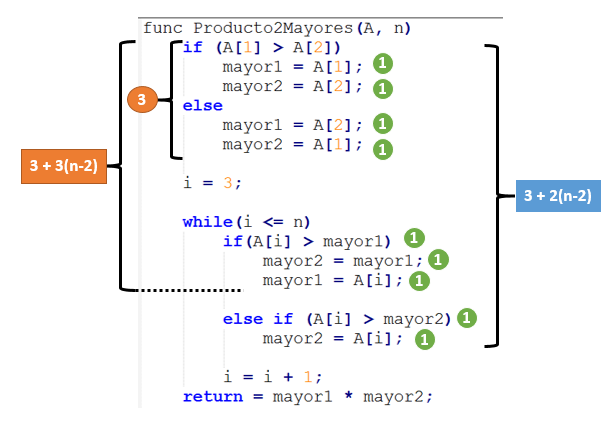
\includegraphics[width=\textwidth]{Abigail/Images/EJER9.PNG}
	 		    \end{figure} 

    			\textbf{Mejor caso} \\
    			\noindent El mejor caso sucede cuando los dos números mayores son los primeros en el arreglo. Entonces observando la imagen, siempre hará $3$ operaciones, más el número de veces que comparara el resto del arreglo. Tenemos la siguiente función:

    			$$
    				f_{tM}(n) = 3 + 2(n - 2)
    			$$

    			\textbf{Peor caso} \\
    			\noindent Caemos en el peor caso cuando los dos números mayores estan hasta el final del arreglo. En dado caso tendremos la siguiente función, que a igual que el mejor caso, siempre se hacen las $3$ primeras operaciones, más el número de veces que comparara el resto del arreglo. Tenemos la siguiente función:

    			$$
    				f_{tP}(n) = 3 + 3(n - 2)	
    			$$
				
				\textbf{Caso medio} \\
				$$ f_{cm}(n) = \frac{8}{3}n - \frac{7}{3} $$
				\noindent 

	        \subsection{Capturas de comprobación}

	        \subsubsection{Código}
	            \begin{lstlisting}[style=Java]
    		    \end{lstlisting}

	% ----------------------------------------------------------------------
	% 															EJERCICIO 10
	% ----------------------------------------------------------------------
	    \subsection{Ejercicio 10}	 

	    \textbf{Operaciones básicas:} Se tomaran en cuenta las operaciones de comparación entre elementos del arreglo, asiganaciones a la variable \textbf{temp} y arreglo a.

			\subsubsection{Algoritmo}
			    \begin{lstlisting}[style=Java]
	    }
func OrdenamientoIntercambio(a, n)	
for(i = 0; i < n-1; i++)
	for(int j = i + 1; j < n; j++)
		if(a[j] < a[i])
		{	temp = a[i];
			a[i] = a[j];
			a[j] = temp;
		}
fin
    		    \end{lstlisting}

    		\subsubsection{Análisis}

	    		\begin{figure}[h!]
	                \centering
	                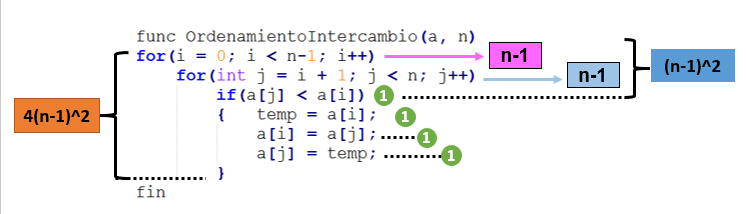
\includegraphics[width=\textwidth]{Abigail/Images/EJER10.PNG}
	 		    \end{figure} 

	    		\begin{itemize}
	    			\item[\Checklist] Mejor caso \\
	    			Ocurre cuando los números ya estan ordenados, entonces solo se llega hasta el \textbf{if} y nunca se cumple la condición, por lo tanto la función es:
	    			$$
	    				f_{tM} = (n-1)^{2}
	    			$$
	    			\item[\Checklist] Peor caso \\
					Tenemos este caso cuando los números estan ordenados de forma \textbf{DESCENDENTE}. En este caso la condición \textbf{if} siempre se cumple y realiza $4$ operaciones, por lo tanto la función es:
					$$
						f_{tP} = 4(n-1)^{2}
					$$
 
					\item[\Checklist] Caso medio \\
					$$
						f_{cm} = \frac{5}{2}(n-1)^{2}	
					$$
				\end{itemize}
	        \subsection{Capturas de comprobación}

	        \subsubsection{Código}
	            \begin{lstlisting}[style=Java]
    		    \end{lstlisting}

	% ----------------------------------------------------------------------
	% 															EJERCICIO 11
	% ----------------------------------------------------------------------

	% NO EXISTEEEEEEEEEEEEEEEEEEEEEEE
	
	% ----------------------------------------------------------------------
	% 															EJERCICIO 12
	% ----------------------------------------------------------------------
	    \subsection{Ejercicio 12}
		\textbf{Operaciones básicas:} Se toman en cuenta la comparación entre los elementos del
		
			\subsubsection{Algoritmo}
			    \begin{lstlisting}[style=Java]
Procedimiento BurbujaOptimizada(int A[], int n)	
	cambios = "No";
	i = 0;
	while((i < n-1) && (cambios != "No"))
	{
		cambios = "No";
		for(j=0; j<=(n-2)-i; j++)
		{
			if (A[j] > A[j+1])
			{
				aux = A[j];
				A[j] = A[i];
				A[i] = aux;
				cambios = "Si";
			}
		}
		i++;
	}
Fin Procedimiento 
    		    \end{lstlisting}

	        \subsubsection{Análisis}

		        \begin{figure}[h!]
	                \centering
	                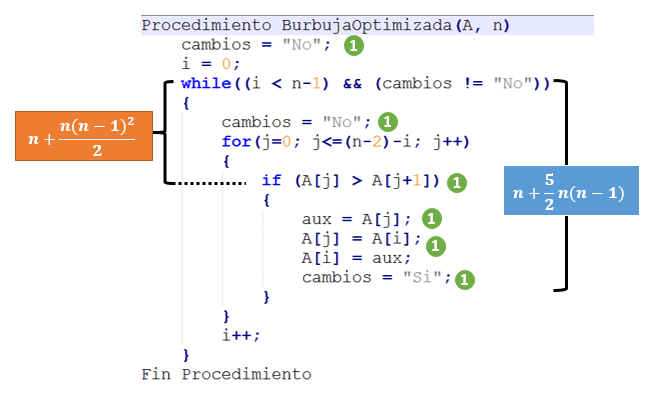
\includegraphics[width=\textwidth]{Abigail/Images/EJER12.PNG}
	 		    \end{figure} 

	    		\begin{itemize}
	    			\item[\Checklist] Mejor caso \\
	    			Sucede cuando los números están ordenados de forma ascendente.

	    			$$
	    				f_{tM} = n + \frac{n(n-1)^{2}}{2}
	    			$$
	    			\item[\Checklist] Peor caso \\
					Ocurre cuando los números estan ordenados de forma descendente.
	    			$$
	    				f_{tP} = n + \frac{5}{2}n(n-1)^{2}
	    			$$

					\item[\Checklist] Caso medio \\
					$$
						f_{cm} = n + \frac{3}{2}n(n-1)^{2}
					$$
				\end{itemize}
	        \subsection{Capturas de comprobación}

	        \subsubsection{Código}
	            \begin{lstlisting}[style=Java]
    		    \end{lstlisting}

	% ----------------------------------------------------------------------
	% 															EJERCICIO 13
	% ----------------------------------------------------------------------
	    \subsection{Ejercicio 13}
		\textbf{Operaciones básicas:} Las comparaciones entre los elementos del arreglo A y las asignaciones a aux y al arreglo.

			\subsubsection{Algoritmo}
			    \begin{lstlisting}[style=Java]
Procedimiento BurbujaSimple(A, n)
	{
		for(i = 0; i <= n-2; i++)
		{
			for(j = 0; j <= (n-2)-i; j++)
			{
				if (A[j] > A[j+1])
				{
					aux = A[j];
					A[j] = A[j+1];
					A[j+1] = aux;
				}
			}
		}
	}
Fin Procedimiento
    		    \end{lstlisting}

	        \subsubsection{Análisis}

		        \begin{figure}[h!]
	                \centering
	                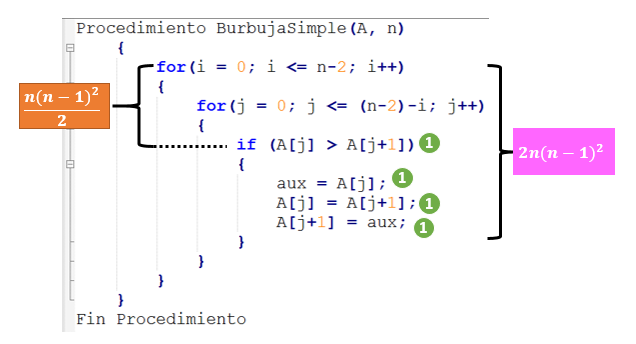
\includegraphics[width=\textwidth]{Abigail/Images/EJER13.PNG}
	 		    \end{figure} 

	    		\begin{itemize}
	    			\item[\Checklist] Mejor caso \\
	    			Sucede cuando los números estan ordenados de manera ascendente.

	    			$$
	    				f_{tM} = \frac{n(n-1)^{2}}{2}
	    			$$

	    			\item[\Checklist] Peor caso \\
					Ocurre cuando los números están desordenados de forma descendente.
					$$
						f_{tP} = 2n(n-1)^{2}
					$$
					\item[\Checklist] Caso medio \\
					$$
						f_{cm} = 5n(n-1)^{2}
					$$

				\end{itemize}	        
	        \subsection{Capturas de comprobación}

	        \subsubsection{Código}
	            \begin{lstlisting}[style=Java]
    		    \end{lstlisting}

	% ----------------------------------------------------------------------
	% 															EJERCICIO 14
	% ----------------------------------------------------------------------
	    \subsection{Ejercicio 14}
		\textbf{Operaciones básicas:} Se toman en cuenta las comparaciones entre a, b y c.
			\subsubsection{Algoritmo}
			    \begin{lstlisting}[style=Java]
Procedimiento Ordena(a, b, c)
{
	if(a > b)
		if(a > c)
			if(b > c)
				salida (a, b, c);
			else
				salida (a, c, b);		
		else
			salida (c, a, b);
	else
		if(b > c)
			if(a > c)
				salida(b, a, c);
			else
				salida(b, c, a);
		else
			salida(c, b, a);
} 
    		    \end{lstlisting}

	        \subsubsection{Análisis}

		        \begin{figure}[h!]
	                \centering
	                \includegraphics[width=\textwidth]{Abigail/Images/EJER14.PNG}
	 		    \end{figure} 
	    		\begin{itemize}
	    			\item[\Checklist] Mejor caso \\
	    			Cuando $ a>b>c $. 
	    			$$
	    				f_{tM} = 2
	    			$$
	    			\item[\Checklist] Peor caso \\
					Cuando $ c>b>a $. 
	    			$$
	    				f_{tP} = 5
	    			$$
	    			
					\item[\Checklist] Caso medio \\
					$$
						f_{cm} = 4
					$$

				\end{itemize}

	        \subsection{Capturas de comprobación}

	        \subsubsection{Código}
	            \begin{lstlisting}[style=Java]
    		    \end{lstlisting}

	% ----------------------------------------------------------------------
	% 															EJERCICIO 15
	% ----------------------------------------------------------------------
	    \subsection{Ejercicio 15}
	   	\textbf{Operaciones básicas:}
		
			\subsubsection{Algoritmo}
			    \begin{lstlisting}[style=Java]
Procedimiento Seleccion(A, n)
	{
		for(k=0; k<n-2; k++)
		{
			p=k;
			for(i = k+1; i<n-1; i++)
			{
				if(A[i] < A[p])
					p = i;
			}
			temp = A[p];
			A[p] = A[k];
			A[k] = temp;
		}
	}
Fin Procedimiento
    		    \end{lstlisting}

	        \subsubsection{Análisis}

		        \begin{figure}[h!]
	                \centering
	                \includegraphics[width=\textwidth]{Abigail/Images/EJER15.PNG}
	 		    \end{figure} 
	    		\begin{itemize}
	    			\item[\Checklist] Mejor caso \\

	    			\item[\Checklist] Peor caso \\
					
					\item[\Checklist] Caso medio \\

				\end{itemize}

	        \subsection{Capturas de comprobación}

	        \subsubsection{Código}
	            \begin{lstlisting}[style=Java]
    		    \end{lstlisting}

\end{document}